\chapter{Parameter Values Distributions in Terms of Quality}\label{appendix:Distributions3}
More plots on \url{https://github.com/RomanKosovnenko/master_thesis/tree/master/images/DistrObj}
\begin{figure}[!htb]
	\centering
	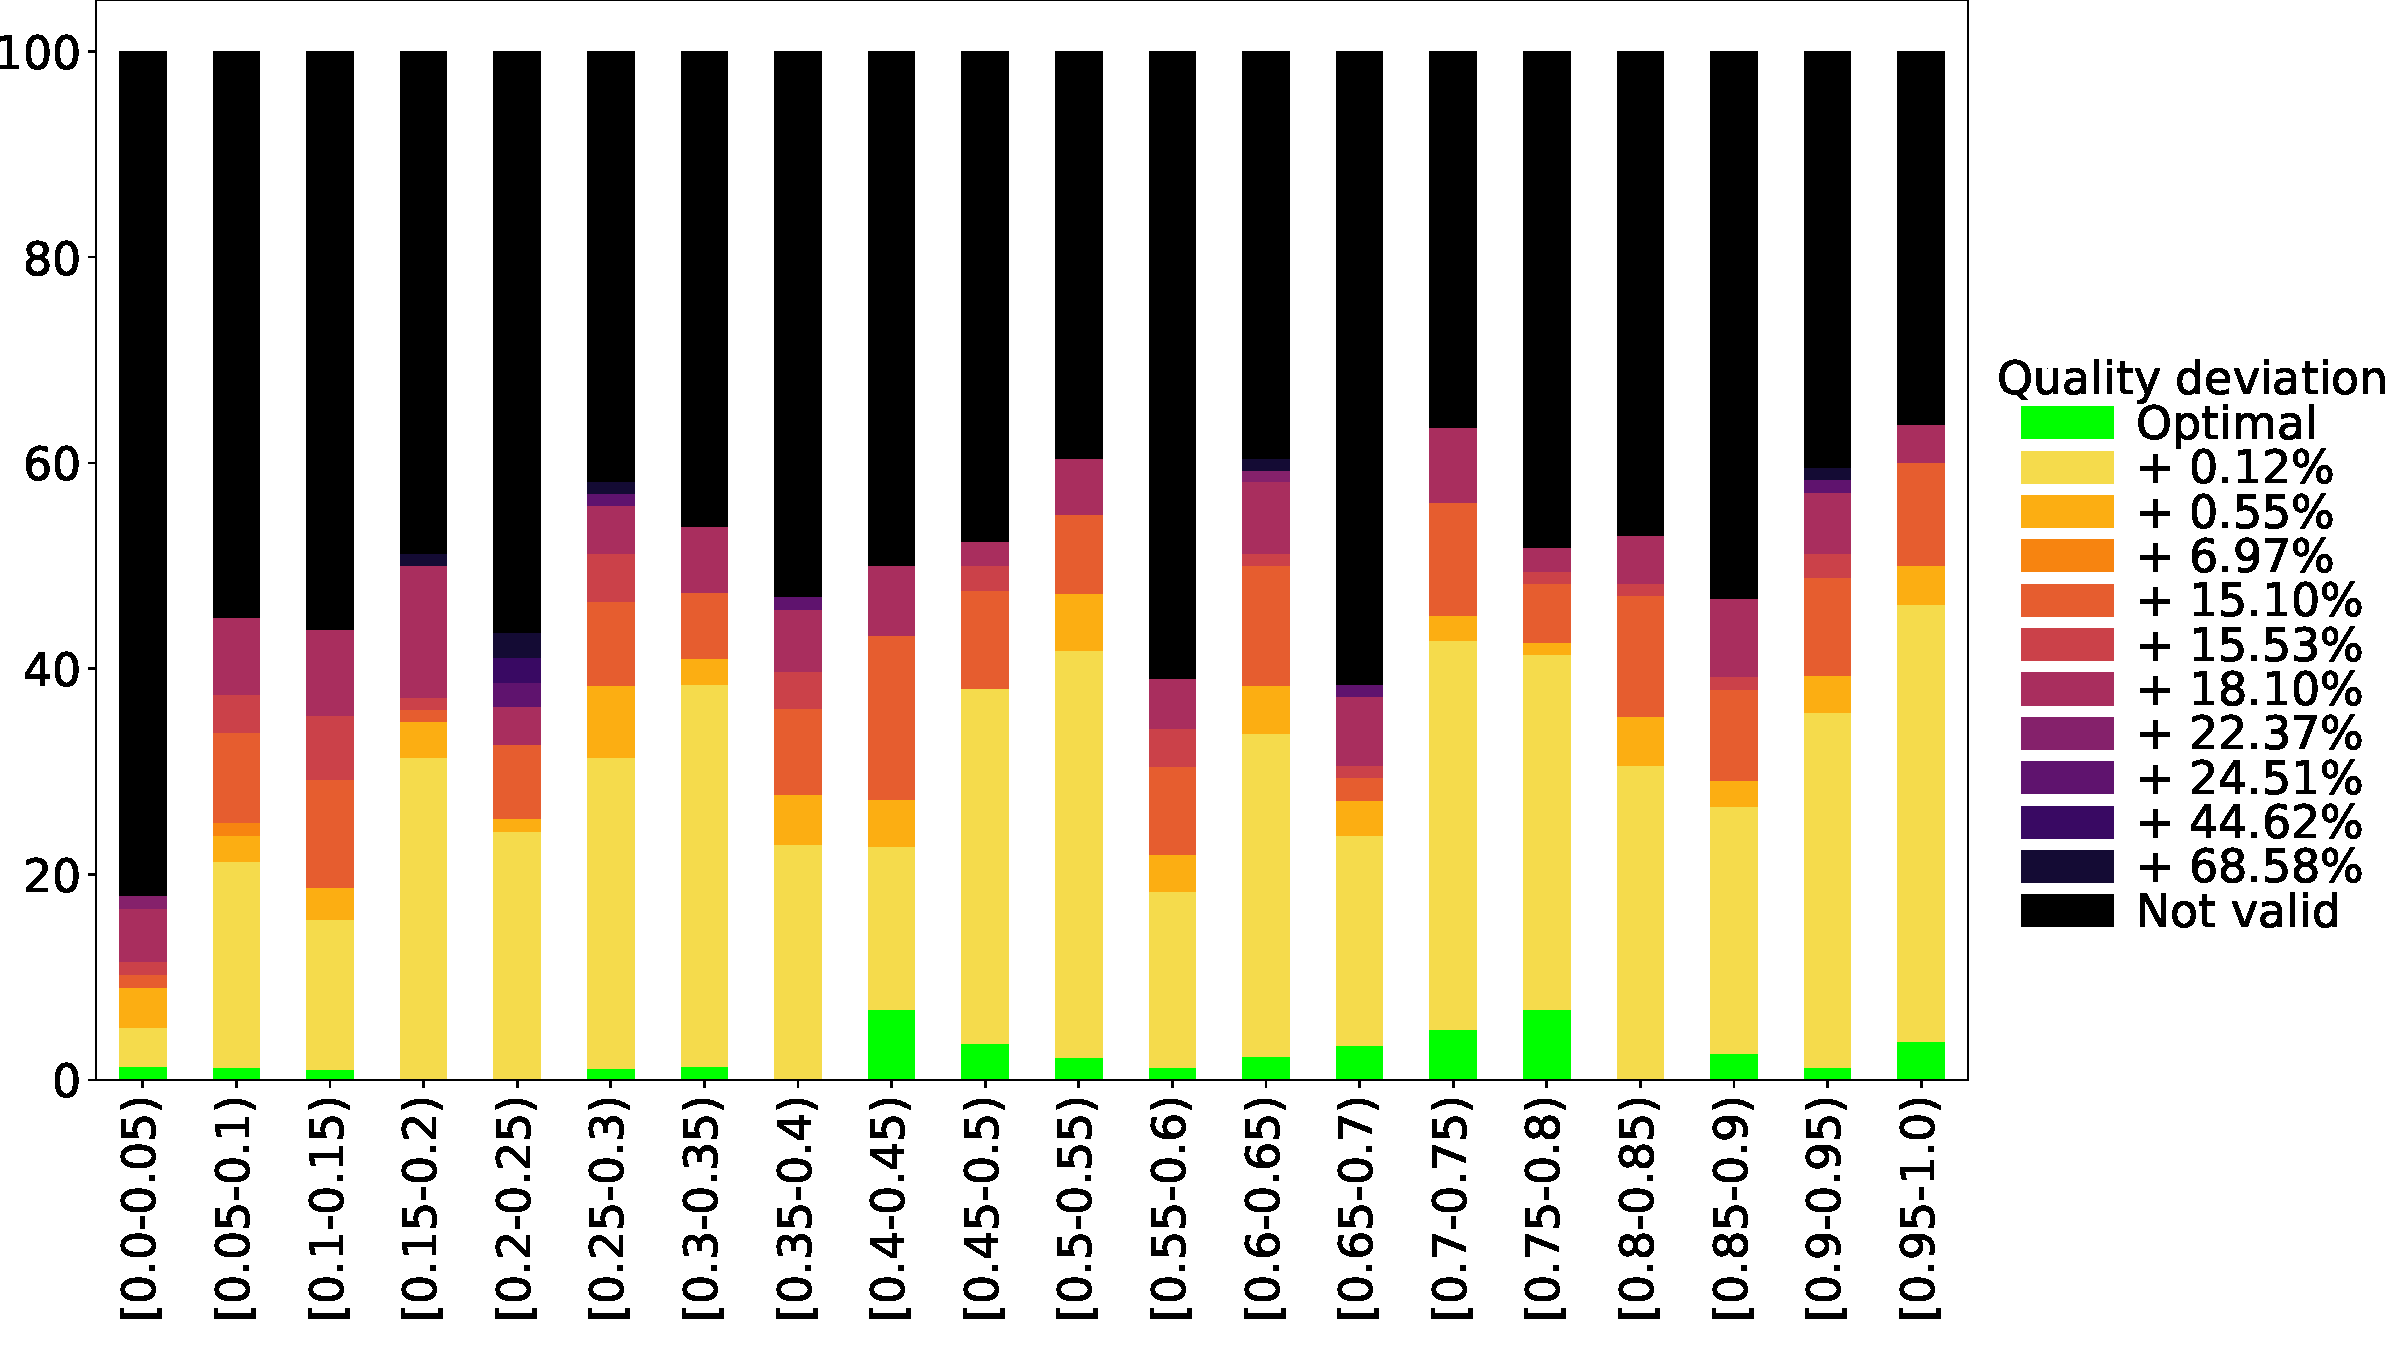
\includegraphics[width=\textwidth]{images/DistrObj/lambda.pdf}
	\caption[]{lambda parameter values distribution for smaller problem}
	\label{fig:lambda_Obj}
\end{figure}

\begin{figure}
	\centering
	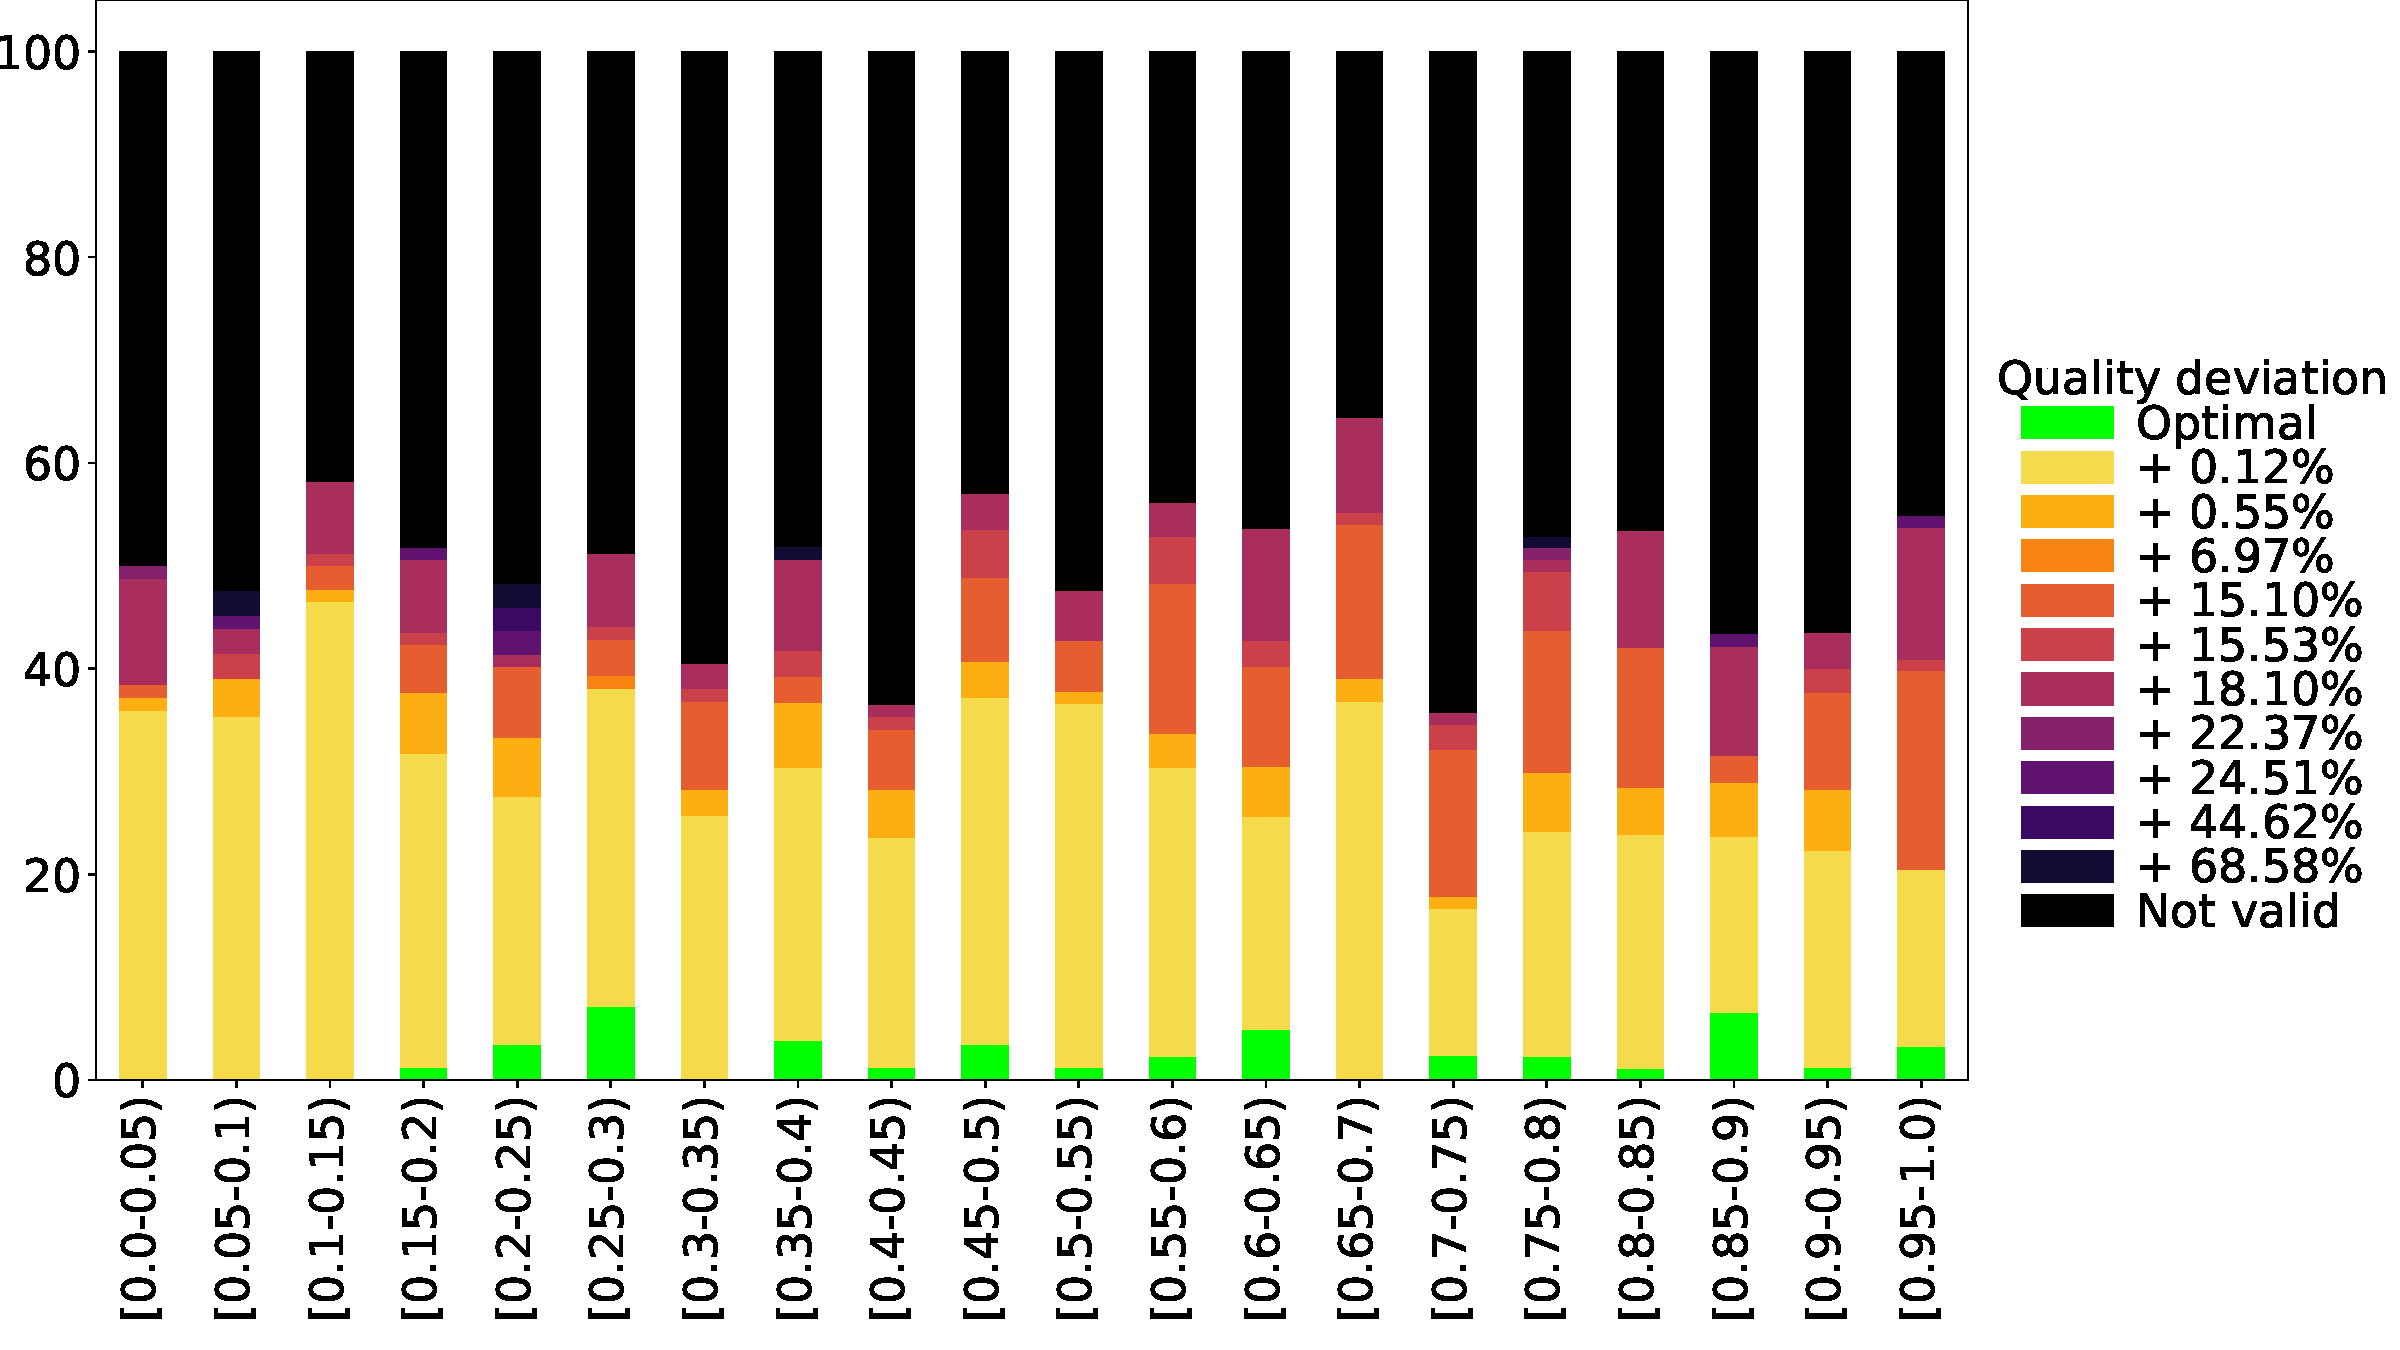
\includegraphics[width=\textwidth]{images/DistrObj/crossoverRate.pdf}
	\caption[]{crossoverRate parameter values distribution for smaller problem}  
	\label{fig:crossoverRate_Obj}
\end{figure}

\begin{figure}
	\centering
	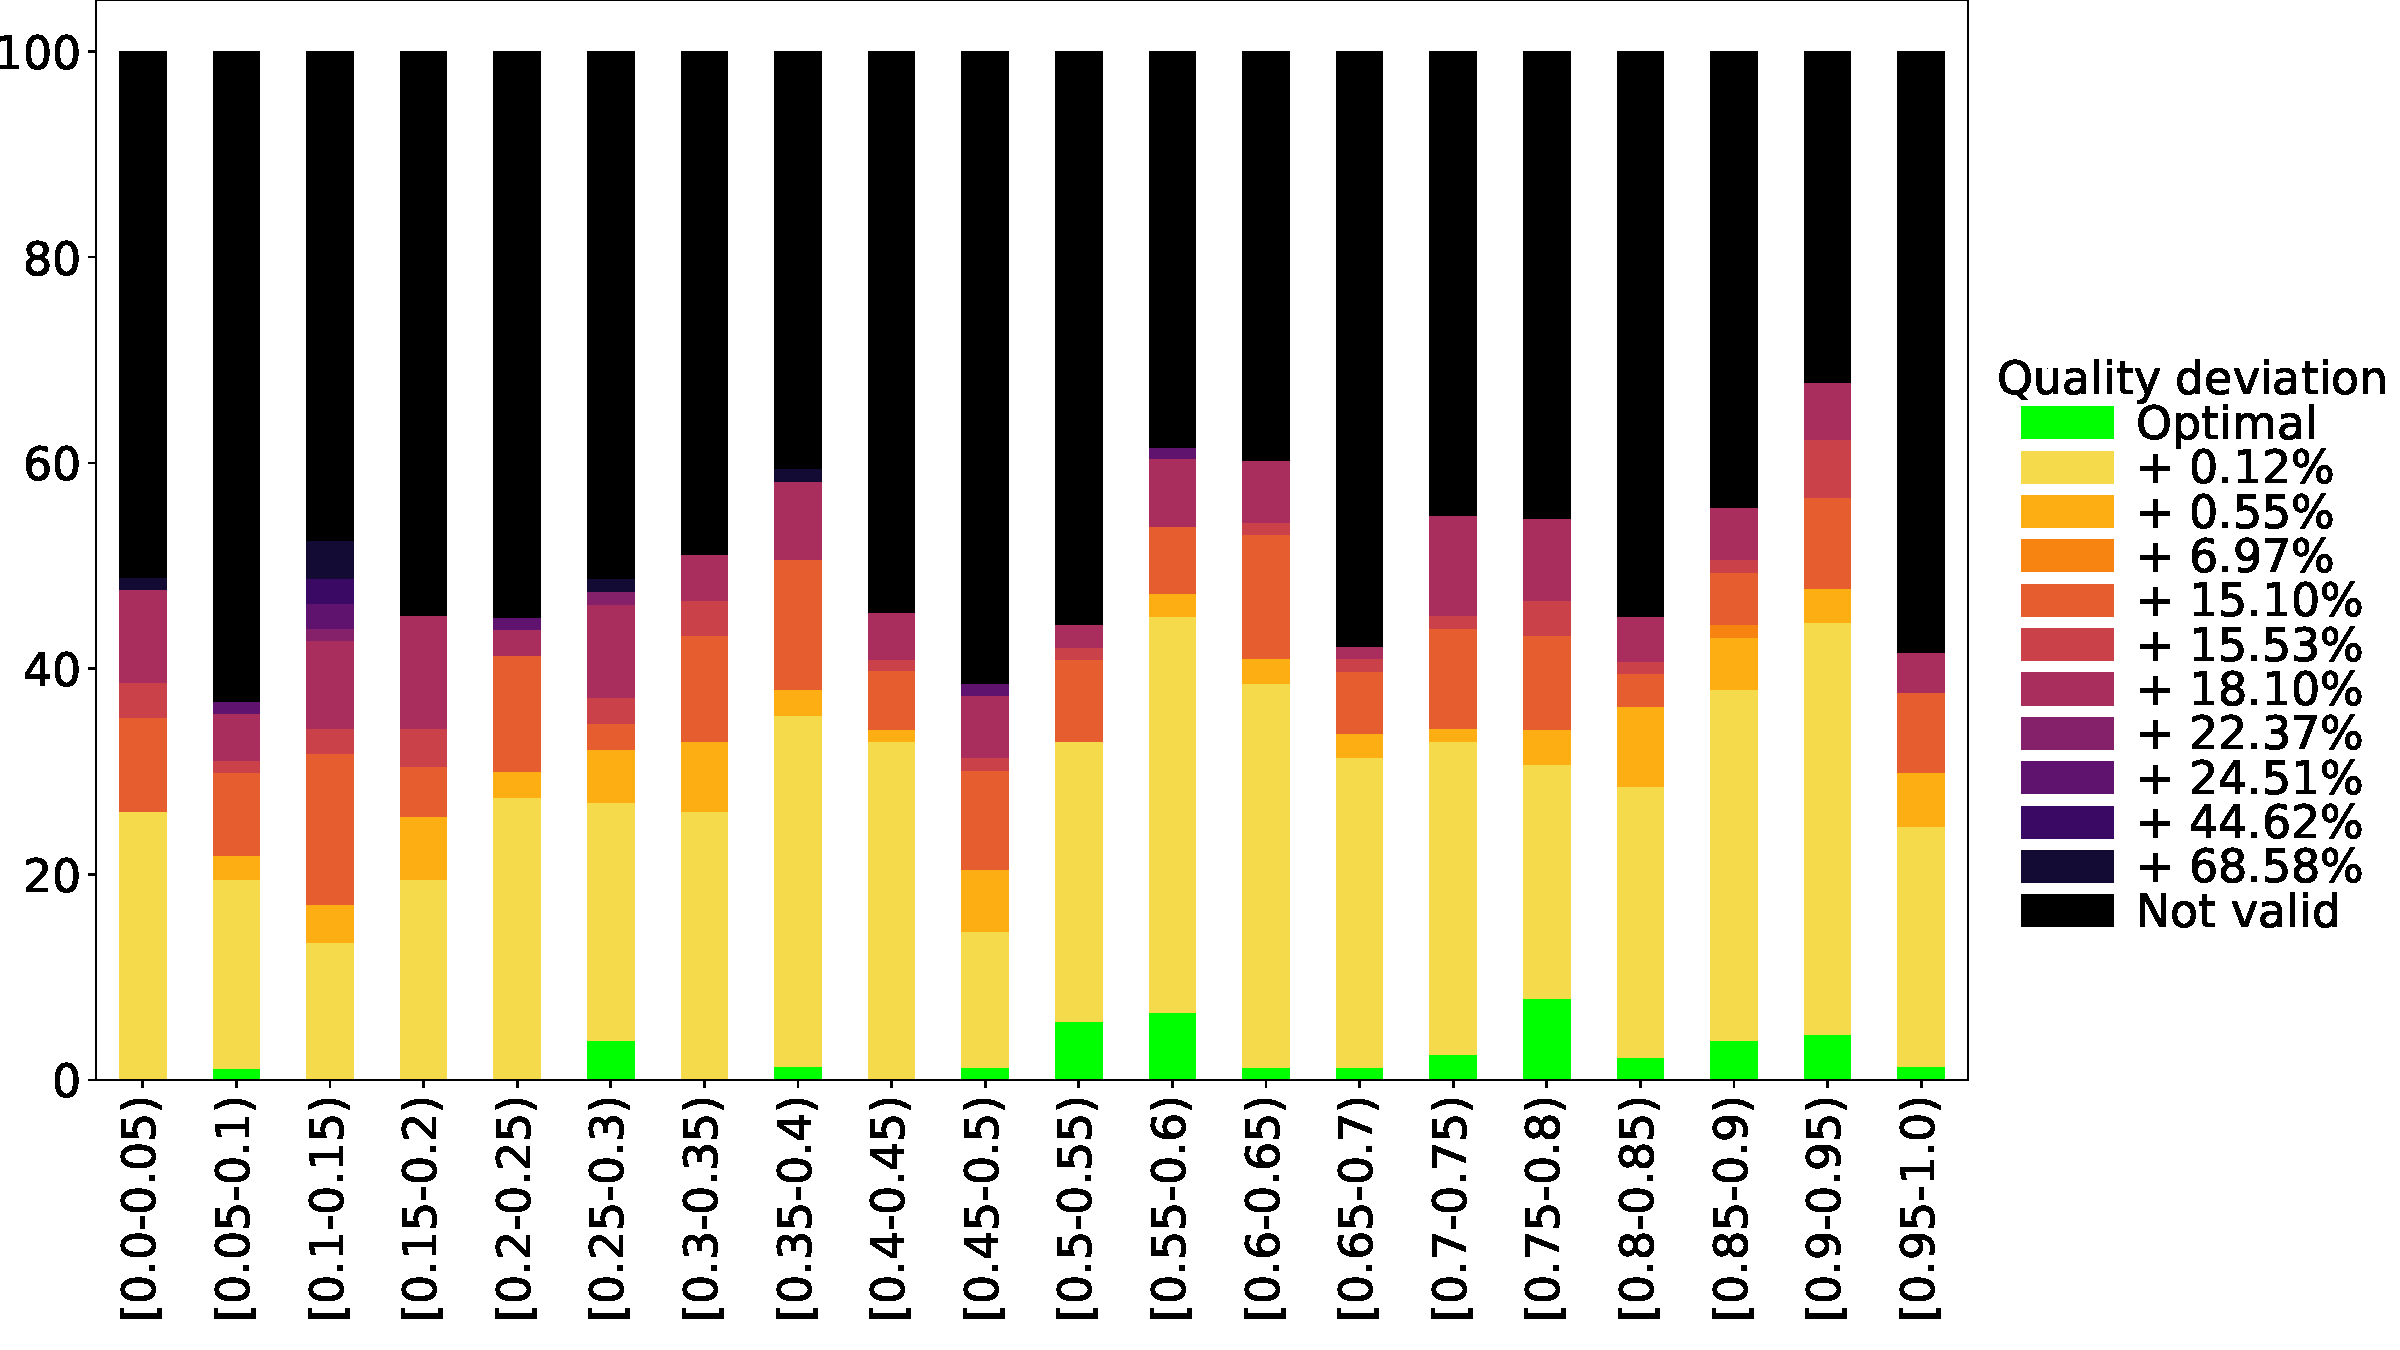
\includegraphics[width=\textwidth]{images/DistrObj/resourcesMutationProbability.pdf}
	\caption[]{resourcesMutationProbability parameter values distribution for smaller problem}
	\label{fig:resourcesMutationProbability_Obj}
\end{figure}

\begin{figure}
	\centering
	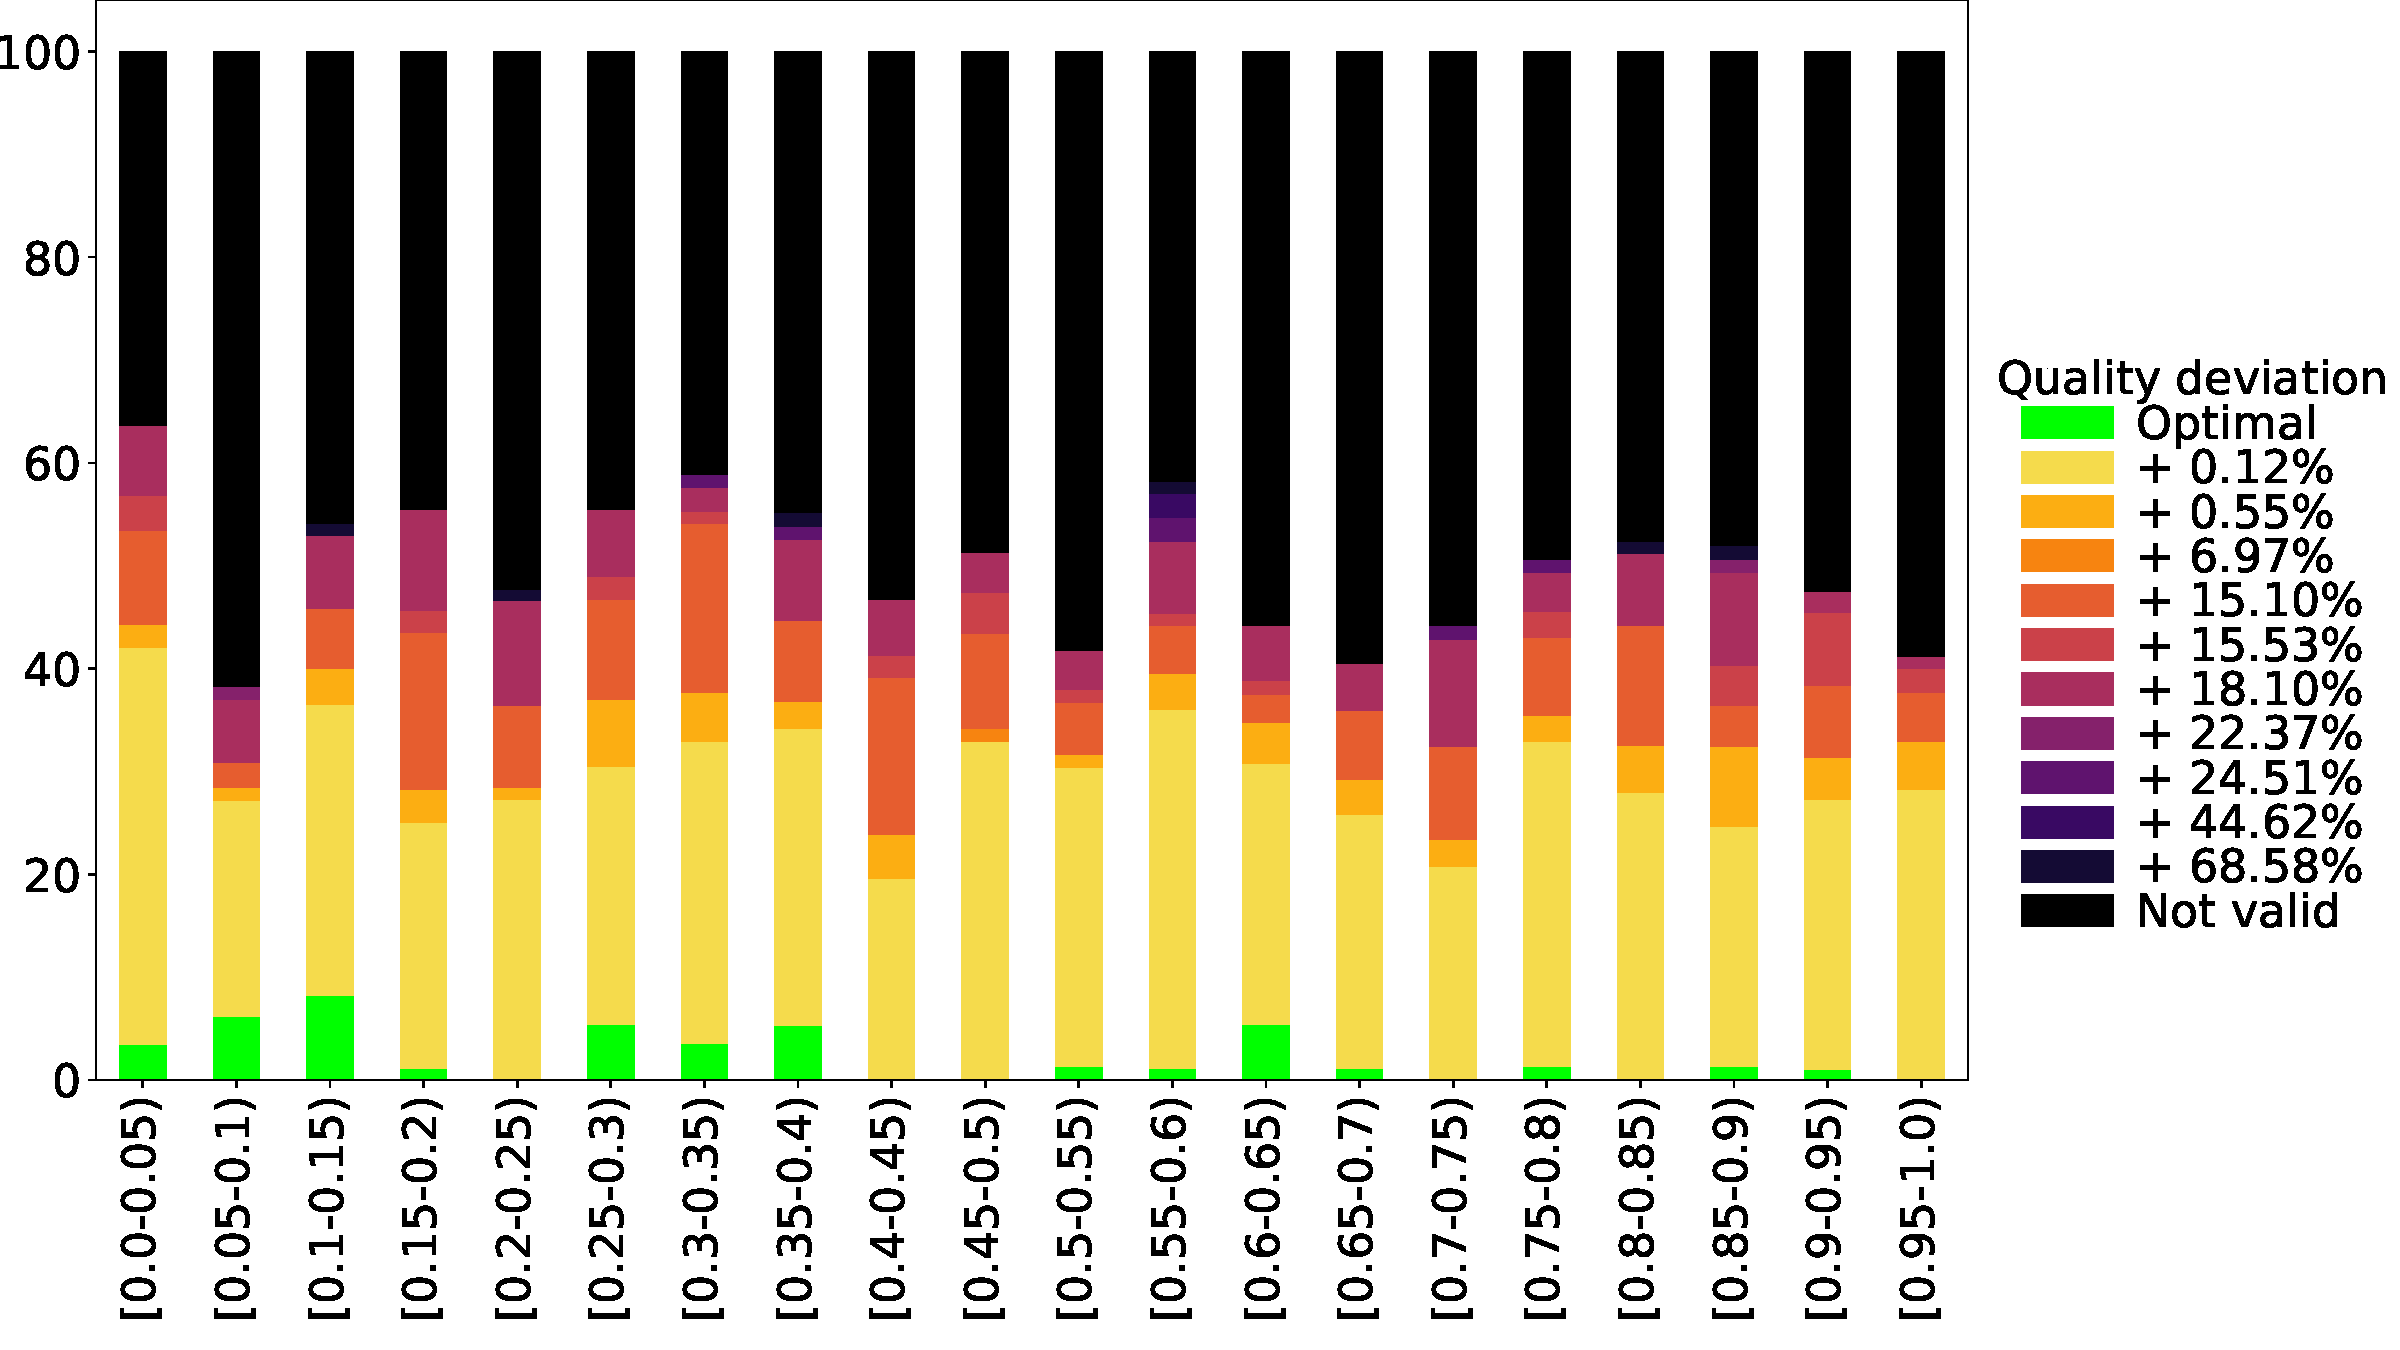
\includegraphics[width=\textwidth]{images/DistrObj/crossoverOnRandomRequestProbability.pdf}
	\caption[]{crossoverOnRandomRequestProbability parameter values distribution for smaller problem}       
	\label{fig:crossoverOnRandomRequestProbability_Obj}
\end{figure}


\begin{figure}
	\centering
	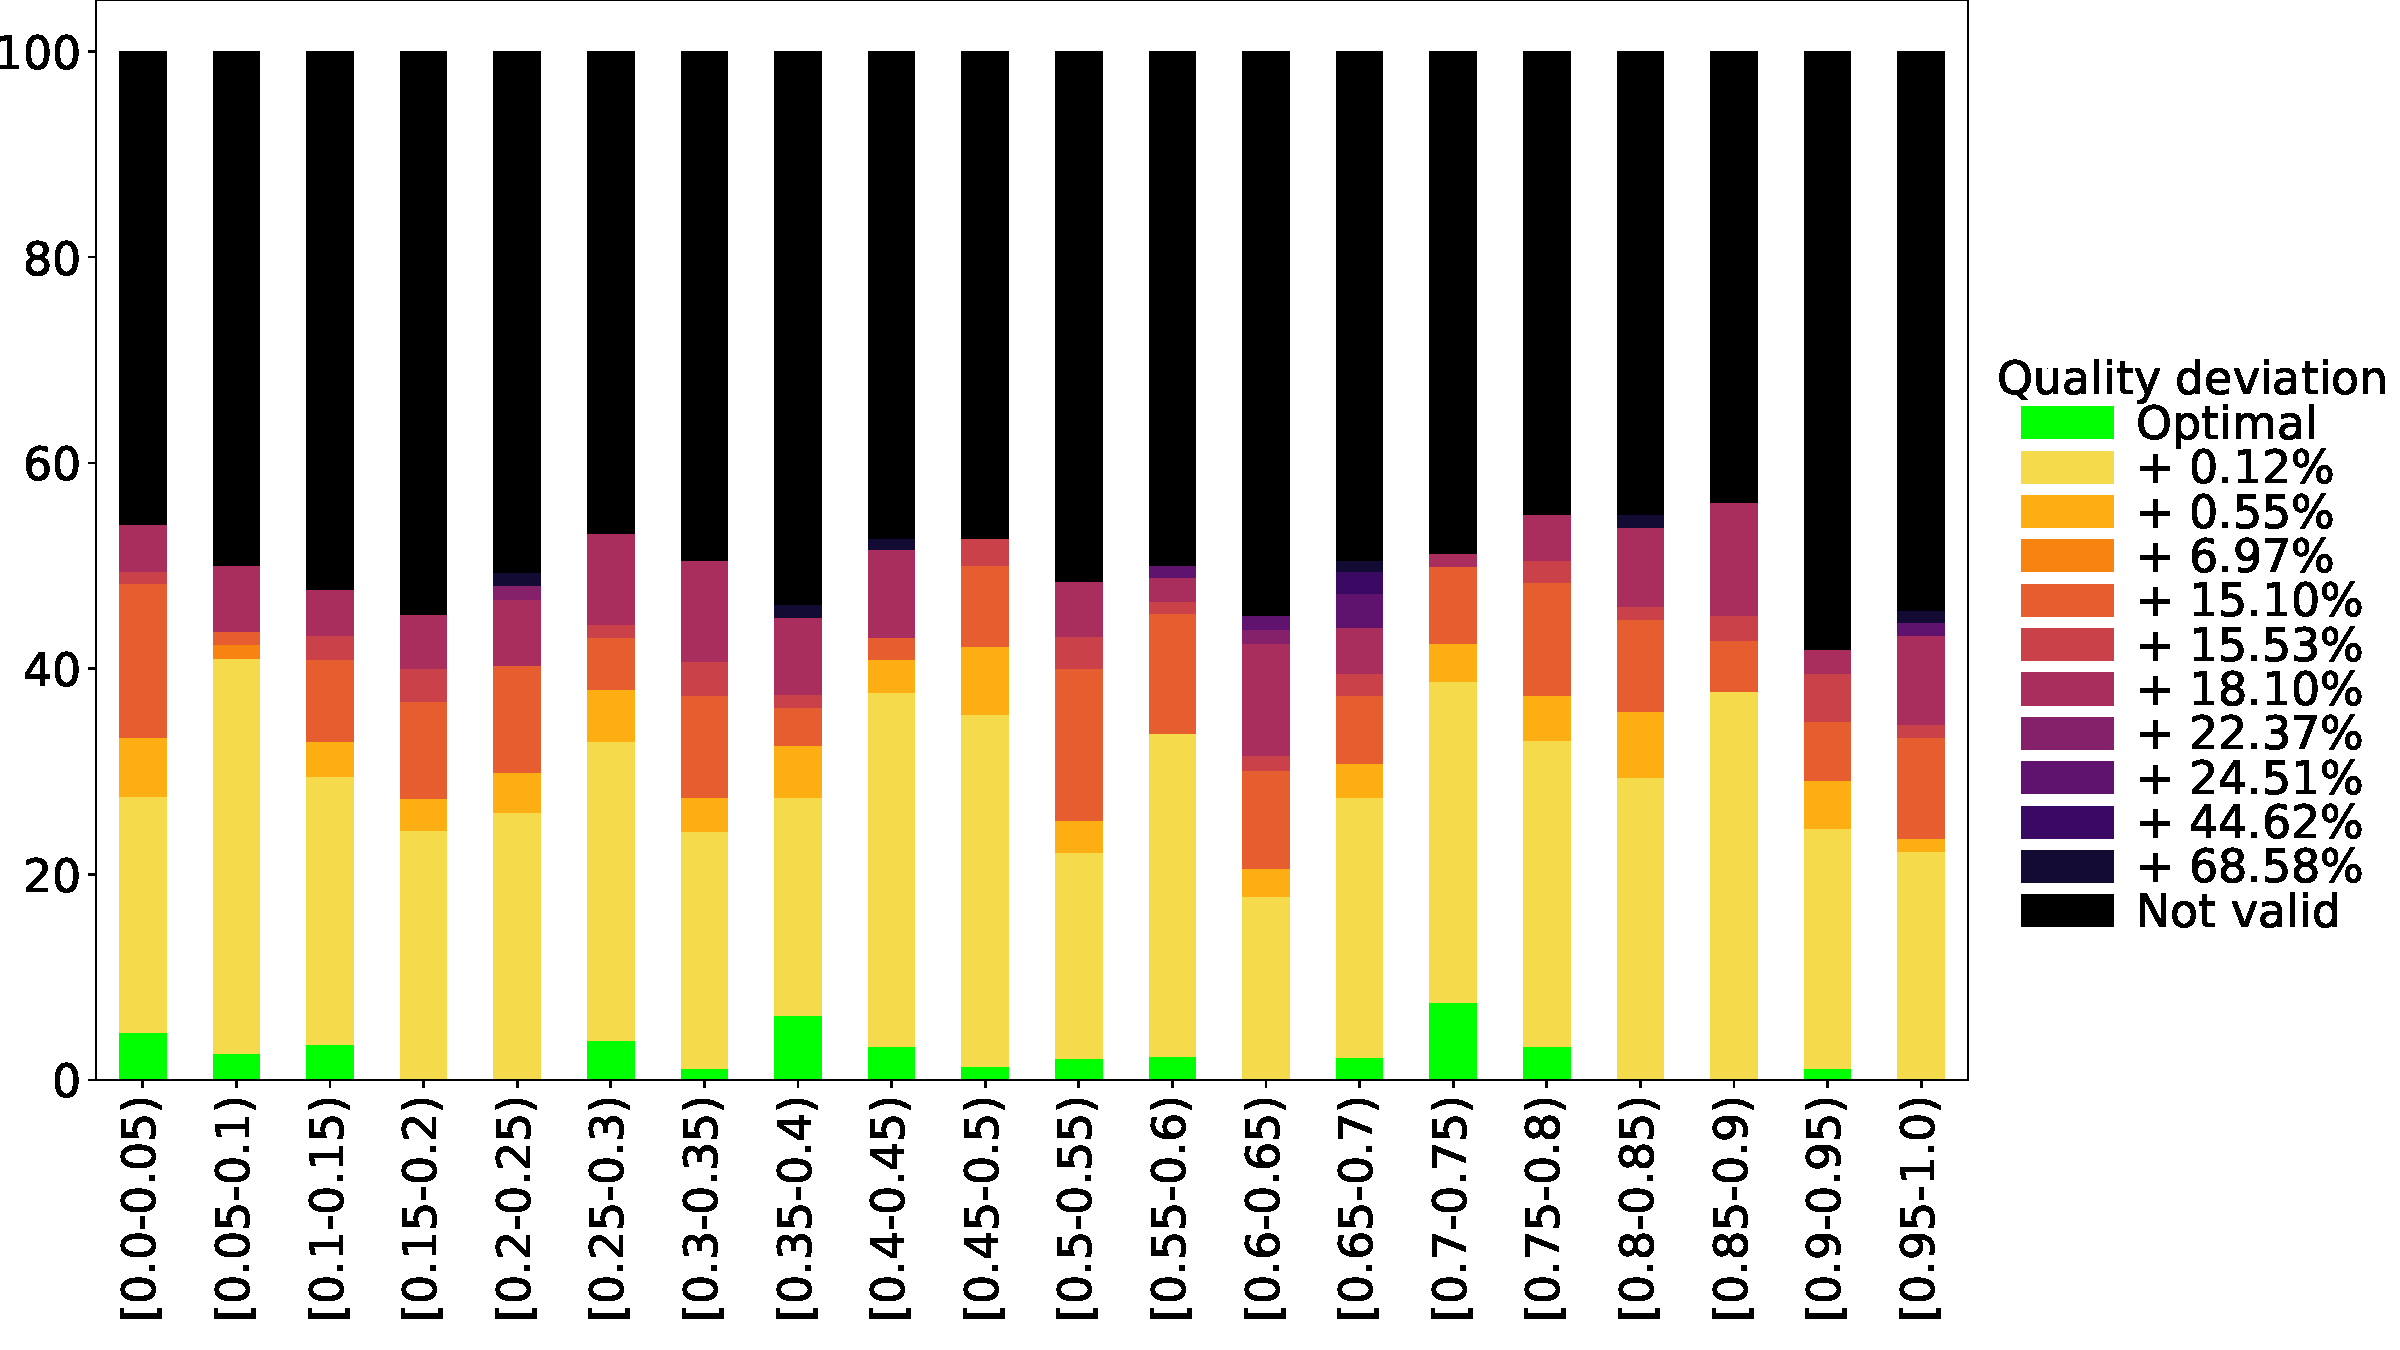
\includegraphics[width=\textwidth]{images/DistrObj/evaluatorValidityWeight.pdf}
	\caption[]{evaluatorValidityWeight parameter values distribution for smaller problem}
	\label{fig:evaluatorValidityWeight_Obj}
\end{figure}

